\documentclass[UTF8,11pt,a4paper,fontset=fandol]{ctexart}

\usepackage[a4paper,margin=2.25cm,headheight=14pt]{geometry}
\usepackage{amsmath,amssymb,bm}
\usepackage{booktabs,tabularx,array,longtable,multirow}
\usepackage{graphicx,float,caption,subcaption}
\usepackage{xcolor}
\usepackage{enumitem}
\usepackage{siunitx}
\usepackage{fancyhdr,lastpage}
\usepackage{microtype}
\usepackage{hyperref}
\usepackage[nameinlink,noabbrev]{cleveref}
\usepackage[backend=biber,style=numeric,sorting=none,maxbibnames=9]{biblatex}

\addbibresource{references.bib}
\graphicspath{{figures/}}

\definecolor{navy}{HTML}{17365D}
\definecolor{blue}{HTML}{2F75B5}
\definecolor{lightblue}{HTML}{DDEBF7}
\definecolor{orange}{HTML}{ED7D31}
\definecolor{todored}{HTML}{C00000}
\hypersetup{
  colorlinks=true,
  linkcolor=navy,
  citecolor=blue,
  urlcolor=blue,
  pdftitle={基于动态边卷积与迭代位移场的点云降噪方法},
  pdfsubject={计图大赛赛道二比赛报告}
}

\pagestyle{fancy}
\fancyhf{}
\fancyhead[L]{基于动态边卷积与迭代位移场的点云降噪方法}
\fancyhead[R]{计图大赛赛道二}
\fancyfoot[C]{\thepage/\pageref{LastPage}}

\setlength{\parindent}{2em}
\setlength{\parskip}{0.25em}
\setlist{nosep,leftmargin=2em}
\renewcommand{\arraystretch}{1.18}
\newcolumntype{Y}{>{\raggedright\arraybackslash}X}
\newcommand{\code}[1]{\texttt{\detokenize{#1}}}
\newcommand{\TODO}[1]{\textcolor{todored}{\textbf{TODO：#1}}}
\setlength{\emergencystretch}{3em}
\AtBeginBibliography{\small\sloppy}
\crefname{figure}{图}{图}
\crefname{table}{表}{表}
\crefname{equation}{式}{式}

\title{\heiti\bfseries 基于动态边卷积与迭代位移场的点云降噪方法\\[0.5em]
\Large 计图大赛赛道二比赛报告}
\author{队伍：alpha奶龙\\[0.4em]
成员：陈梓扬，李成蹊，黄元涛}
\date{\today}

\begin{document}

\maketitle
\thispagestyle{empty}
\vfill
\begin{center}
\begin{minipage}{0.88\textwidth}
\small
\textbf{报告口径说明：}本文以 GitHub 仓库 \url{https://github.com/LiChengxi666/denoise_jittor}
的 \code{vm_strong} 分支为准，仅描述 \code{starter_code/} 中实际启用的 strong 路线。
默认训练/推理入口分别为 \code{configs/task/train_vm.yaml} 与
\code{configs/task/predict_vm.yaml}，二者均指向 \code{vm_strong} 组件。
仓库中的 sprint、recovery、InfoCD、独立 CD 邻域、排斥/尺度约束和增强 P2S 代理损失属于
后续实验能力，不作为最终方案或已验证收益进行陈述。训练与评测日志保存在云服务器，
本地仓库默认不包含完整 \code{metrics.csv}；最终权重按固定验证集表现选择，但现有材料
不足以建立某个具体 checkpoint 与最终榜单成绩的一一对应关系。训练曲线中，1--10 epoch 逐轮
损失来自同步日志；各 checkpoint 对应 epoch 的验证损失视为已知锚点；连续趋势线为对这些
锚点的拟合，不代表逐 epoch 实测。
\end{minipage}
\end{center}
\vfill
\clearpage

\begin{abstract}
本文面向计图大赛赛道二的点云降噪任务，在官方 StraightPCF 风格 baseline 上实现并提交了
\code{vm_strong} 路线。方法以含噪点云与干净点云之间的随机混合状态为输入，利用三层动态边卷积
提取局部几何特征，并将全局最大池化特征广播到每个点，通过多层感知机预测逐点三维位移。
训练目标联合位移回归、双向 Chamfer 距离、点到局部切平面距离和位移幅值正则，从点对应、集合覆盖
和曲面贴合三个层面约束结果。推理阶段保持原始测试坐标与点数不变，采用最远点采样构造重叠邻域，
执行多轮局部迭代更新，再以中心距离权重融合重叠预测。工程侧在 \code{vm_strong} 分支上建立了
配置化训练、云端日志、固定验证集 CD/P2S 选模、输出格式检查和提交包审计闭环。
现存提交包共含 200 个预测文件，均与输入保持 $50\,000\times3$、\texttt{float32} 和有限数值约束。
最终 A 榜提交采用 E9 推理配置（\code{checkpoint_39.pkl}，\code{predict_step_size=0.97}、
\code{predict_momentum=0.6}、\code{predict_patch_weight_gamma=4.0}、线性步长衰减、外步 2），
官网总分为 \textbf{74.16}（CD \textbf{62.36}，P2S \textbf{85.95}），截至 2026-06-28 22:05
排名第 \textbf{36} 名。

\noindent\textbf{关键词：}点云降噪；vm\_strong；动态边卷积；位移场；Chamfer Distance
\end{abstract}

\tableofcontents
\clearpage

\section{问题背景与任务定义}

点云能够直接表达三维物体表面，但采集过程中的传感器误差、遮挡和环境干扰会使采样点偏离
潜在曲面\cite{wang2026pcdsurvey,hu2026lecture08}。降噪算法既要把点移动回真实表面，
也要避免局部收缩、点聚集与薄结构过平滑。与图像规则网格不同，点云是无序集合，因此模型还需要
同时处理排列不变性、局部邻域构造和大规模点集上的计算开销。

StraightPCF 将含噪 patch 视为噪声端与干净端之间的中间状态，通过 VelocityModule 预测沿
恢复轨迹的常量位移\cite{edirimuni2024straightpcf}；MSPoint 与外部迭代分数模型等工作则进一步
强调多尺度分数估计与外部迭代去噪\cite{hu2023mspoint,guan2025eiscd}。本项目在官方 Jittor
baseline 上沿 StraightPCF 思路扩展 \code{vm_strong} 配置：保留“局部几何编码＋逐点位移预测”
核心路线，并增强模型容量、联合损失与迭代推理策略。

\subsection{输入、输出与数据限制}

训练集只使用比赛提供的 ShapeNet 干净网格，其路径结构为
\begin{center}
\small\nolinkurl{dataset_train/shapenet/<synset_id>/<model_id>/models/model_normalized.obj}。
\end{center}
测试输入文件为 \code{noisy.npy}，数据类型为 \texttt{float32}，形状为 $(N,3)$。
输出文件为 \code{denoised.npy}，点数、数据类型和三维坐标格式均须与输入一致。
最终压缩包根目录直接包含 \code{shapenet/}，不能引入额外路径层级。
当前 \code{datalist/} 记录了 15,732 个训练对象、99 个验证对象和 200 个测试对象；
训练列表覆盖 13 个 ShapeNet 类别，现存测试包涉及 12 个类别。

\subsection{评价指标}

设预测点集为 $P$，干净参考点集为 $G$。代码中的 Chamfer Distance（CD）使用双向平方
最近邻距离：
\begin{equation}
\operatorname{CD}(P,G)=
\frac{1}{|P|}\sum_{\bm p\in P}\min_{\bm g\in G}\|\bm p-\bm g\|_2^2+
\frac{1}{|G|}\sum_{\bm g\in G}\min_{\bm p\in P}\|\bm g-\bm p\|_2^2.
\label{eq:cd}
\end{equation}
Point-to-Surface Distance（P2S）计算每个预测点到参考三角网格表面的平方距离均值：
\begin{equation}
\operatorname{P2S}(P,\mathcal M)=
\frac{1}{|P|}\sum_{\bm p\in P}\min_{\bm q\in\mathcal M}\|\bm p-\bm q\|_2^2.
\label{eq:p2s}
\end{equation}
本地评测脚本分别比较预测与含噪输入的指标改善比例，并以 CD、P2S 各 50\% 汇总。
CD 反映双向集合覆盖，P2S 更直接衡量点是否回到曲面；二者共同约束可以避免只追求“贴面”
而忽略点分布的退化。由于官方测试真值不可见，本文不将本地合成验证分数冒充官方成绩。

\section{vm\_strong 代码框架与整体流程}

\subsection{Git 演化与默认入口}

\code{vm_strong} 路线在仓库 \code{vm_strong} 分支上迭代，相对官方 starter baseline 的
主要提交节点如\cref{tab:git} 所示。其中 commit \code{0c2552b} 首次引入
\code{configs/model/vm_strong.yaml}、\code{train_vm_strong.yaml} 以及验证/网格选模工具链；
commit \code{a193e8e} 补充云端分段训练脚本与 CD 独立邻域等实验能力；后续 sprint 与
fine-tune 配置保留在同一分支，但不在本文最终方案口径内。

\begin{table}[H]
\centering
\caption{\code{vm_strong} 相对 baseline 的主要 Git 节点（\code{starter_code/}）。}
\label{tab:git}
\small
\begin{tabularx}{\textwidth}{lY}
\toprule
提交 & 主要内容 \\
\midrule
\code{8de9121} & 官方 Jittor StraightPCF 风格 baseline（\code{model/vm.yaml}） \\
\code{0c2552b} & 引入 \code{vm_strong} 模型/训练配置、验证诊断与网格选模工具 \\
\code{a193e8e} & 强化训练/评测管线，新增 \code{scripts/cloud/} 云端分段训练 \\
\code{3aac035} & 基于 \code{checkpoint_39} 的 indclean1600 微调脚本（探索分支） \\
\bottomrule
\end{tabularx}
\end{table}

默认入口通过 task 配置将数据、变换、模型和系统组件绑定到 \code{vm_strong}：
\begin{center}
\small
\begin{tabular}{ll}
\toprule
组件 & 默认配置文件 \\
\midrule
训练 task & \code{configs/task/train_vm.yaml} $\rightarrow$ \code{train_strong} + \code{vm_strong} \\
推理 task & \code{configs/task/predict_vm.yaml} $\rightarrow$ \code{vm_strong} + \code{checkpoint_best.pkl} \\
模型 & \code{configs/model/vm_strong.yaml} \\
变换 & \code{configs/transform/vm_strong.yaml} \\
系统 & \code{configs/system/vm_strong.yaml} \\
\bottomrule
\end{tabular}
\end{center}
旧 baseline 已备份为 \code{train_vm_baseline.yaml} / \code{predict_vm_baseline.yaml}，
便于与 \code{vm_strong} 做结构对照。

\subsection{配置化模块划分}

\code{starter_code/} 采用“task 入口 + 四类组件”的解耦结构：
\begin{itemize}
  \item \textbf{data}：\code{configs/data/train_strong.yaml} 指定 ShapeNet 训练/验证列表；
  \item \textbf{transform}：\code{vm_strong.yaml} 定义采样、归一化、加噪、patch 与 mix 状态构造；
  \item \textbf{model}：\code{VelocityModule}（\code{src/model/vm.py}）封装 EdgeConv 编码器、
        位移解码器、联合损失与 patch 推理；
  \item \textbf{system}：\code{VMSystem}（\code{src/system/vm.py}）负责训练循环、checkpoint 保存
        与 \code{denoised.npy} 写出断言。
\end{itemize}
固定随机种子同时设置 Jittor、NumPy 和 Python 随机源，降低配置比较中的额外波动。

\subsection{端到端数据流}

\cref{fig:overview} 展示了 \code{vm_strong} 从干净网格到训练、推理和提交的完整链路。
训练阶段从网格表面采样点及法向，完成单位球归一化后合成多类型噪声，并裁剪为局部 patch。
网络在随机混合状态上预测回到干净点的位移，通过联合损失优化。推理阶段直接读取比赛提供的
含噪点云，不进行重新采样、归一化或加噪；整云被拆分成重叠 patch，局部预测经加权融合后
恢复原有点序和点数。

\begin{figure}[H]
  \centering
  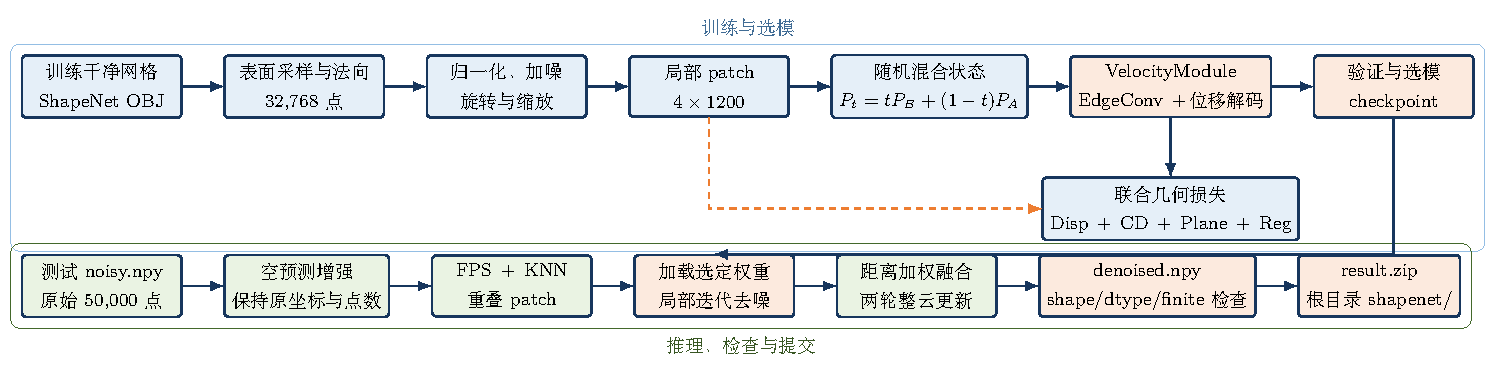
\includegraphics[width=\textwidth]{system_overview.pdf}
  \caption{\code{vm_strong} 训练、验证、推理与提交的整体数据流。虚线表示只在训练阶段使用的干净监督。}
  \label{fig:overview}
\end{figure}

\section{模型结构}

\subsection{动态边卷积特征提取}

对中心点特征 $\bm x_i$ 及其邻点 $\bm x_j$，EdgeConv 消息写为
\begin{equation}
\bm m_{ij}=h_{\theta}\!\left([\bm x_i,\bm x_j-\bm x_i]\right),\qquad
\bm x_i'=\frac{1}{|\mathcal N(i)|}\sum_{j\in\mathcal N(i)}\bm m_{ij}+W\bm x_i.
\label{eq:edgeconv}
\end{equation}
邻域在每一层输入特征上重新执行 $k$ 近邻搜索，因此不仅利用坐标邻接，也能逐层形成语义化
邻域\cite{wang2026pcdsurvey,hu2024pointcloudtech}。
\code{vm_strong} 配置取 $k=24$，三层输出维度依次为 48、96 和 384。第三层输入拼接前两层
特征，兼顾浅层局部细节与较深层几何表示。

\subsection{全局—局部融合与位移解码}

第三层的 384 维逐点特征经过全局最大池化，得到物体级 384 维描述；随后广播到所有点并与
局部特征拼接，形成 768 维条件向量。解码器采用 $768\rightarrow768\rightarrow256
\rightarrow3$ 的全连接结构，前两层使用 Batch Normalization、ReLU 和 0.1 Dropout，最终
输出三维位移。该结构不直接生成新点，而是在输入点上预测偏移，从机制上满足同点数输出约束。

\begin{figure}[H]
  \centering
  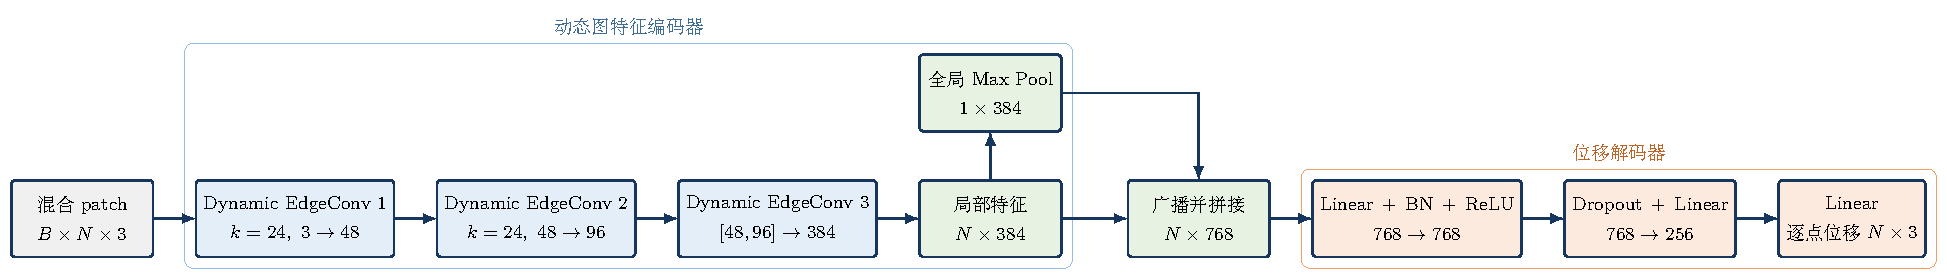
\includegraphics[width=0.96\textwidth]{model_architecture.pdf}
  \caption{\code{vm_strong} 模型结构。动态图在坐标与中间特征上逐层重建，全局特征与局部特征融合后预测逐点位移。}
  \label{fig:model}
\end{figure}

\section{训练策略}

\subsection{网格采样与噪声合成}

每次加载干净网格后共采样 32,768 个点，其中最多 1,024 个点直接来自原网格顶点，其余按
三角面面积进行表面采样，并同步取得法向。点云以包围盒中心平移，再按最远点半径缩放至单位球。
噪声标准差从 $[0.005,0.020]$ 均匀采样，噪声类型在 Gaussian 与等方差 Laplace 分布中随机
选择。训练阶段还以 0.5 概率执行 $[0.8,1.2]$ 的各向同性缩放，以及三个坐标轴上
$[-180^\circ,180^\circ]$ 的随机旋转。最后随机选取 4 个种子，以含噪点云上的 KNN 构造
4 个 1,200 点 patch。验证阶段关闭旋转缩放，但保留采样、归一化、加噪和 patch 构造。
训练 patch 使用随机种子以提升多样性；推理 patch 则改用 FPS 种子以保证整云覆盖均匀。

\subsection{随机混合状态与位移监督}

对于对应的含噪 patch $P_A$ 和干净 patch $P_B$，代码对每个点独立采样
$t\sim\mathcal U(10^{-8},1)$，构造
\begin{equation}
P_t=tP_B+(1-t)P_A,
\label{eq:mix}
\end{equation}
并用同一插值规则得到 patch 种子，将三组点云平移到该种子坐标系。模型输入 $P_t$，目标位移为
\begin{equation}
\bm v^*=P_B-P_t.
\label{eq:target}
\end{equation}
与只在固定噪声端点做回归相比，随机混合状态覆盖了从噪声点到干净点之间的连续位置，使同一个
网络能在迭代推理的中间状态上继续给出更新方向\cite{edirimuni2024straightpcf}。
每个 patch 随机抽取 512 个点参与位移解码和损失计算，以平衡局部覆盖与显存开销。

\subsection{联合损失}

\code{vm_strong} 路线使用四项损失：
\begin{align}
\mathcal L_{\mathrm{disp}}&=\frac{1}{M}\sum_i
\frac{\|\hat{\bm v}_i-\bm v_i^*\|_2^2}{\sigma},\\
\mathcal L_{\mathrm{plane}}&=\frac{1}{M}\sum_i
\frac{\left((\hat{\bm p}_i-\bm p_i^*)^\top\bm n_i\right)^2}{\sigma},\\
\mathcal L_{\mathrm{offset}}&=\frac{1}{M}\sum_i
\frac{\|\hat{\bm v}_i\|_2^2}{\sigma},
\end{align}
其中 $\sigma=0.01$，$\hat{\bm p}_i=P_{t,i}+\hat{\bm v}_i$。集合项
$\mathcal L_{\mathrm{CD}}$ 采用与\cref{eq:cd}相同的双向最近邻结构。总损失为
\begin{equation}
\mathcal L=1.0\mathcal L_{\mathrm{disp}}+0.2\mathcal L_{\mathrm{CD}}
+0.3\mathcal L_{\mathrm{plane}}+0.01\mathcal L_{\mathrm{offset}}.
\label{eq:loss}
\end{equation}
位移项提供强对应监督，CD 关注集合级覆盖，切平面项抑制法向方向的残余噪声，弱位移正则降低
过度修正风险。优化器为 Adam，基础学习率 $3\times10^{-5}$；前 5 个 epoch 线性 warm-up，
之后使用余弦退火至 $3\times10^{-6}$，并将全局梯度范数裁剪到 1.0。

\section{推理与后处理}

预测配置 \code{transform/predict.yaml} 使用空增强列表，因此测试点云不会被训练期的数据处理改变。
设输入点数为 $N$，patch 大小 $M=1200$，重叠系数 $s=6$，patch 数量为
$K=\lceil sN/M\rceil$。算法先用 FPS 在整云上选择 $K$ 个种子，再为每个种子查询 $M$ 个
最近邻，并减去种子坐标完成局部中心化。

每个 patch 内执行 4 次位移更新，总步长配置为 0.8，因此单次更新尺度为 $0.8/4=0.2$。
完整 patch 分解与融合在外层重复 2 轮。重叠区域中，第 $i$ 个 patch 对点 $j$ 的归一化平方
距离记为 $\bar d_{ij}$，融合权重为
\begin{equation}
w_{ij}=\exp(-\gamma\bar d_{ij}),\qquad \gamma=1.
\end{equation}
最终坐标由所有覆盖该点的 patch 预测加权平均得到。中心附近的估计权重更大，从而降低 patch
边界上下文不完整带来的误差。代码中该更新循环命名为 \code{denoise_langevin_dynamics}，
沿用 starter 命名；实现上为确定性位移迭代，不含随机 Langevin 噪声项。

\begin{figure}[H]
  \centering
  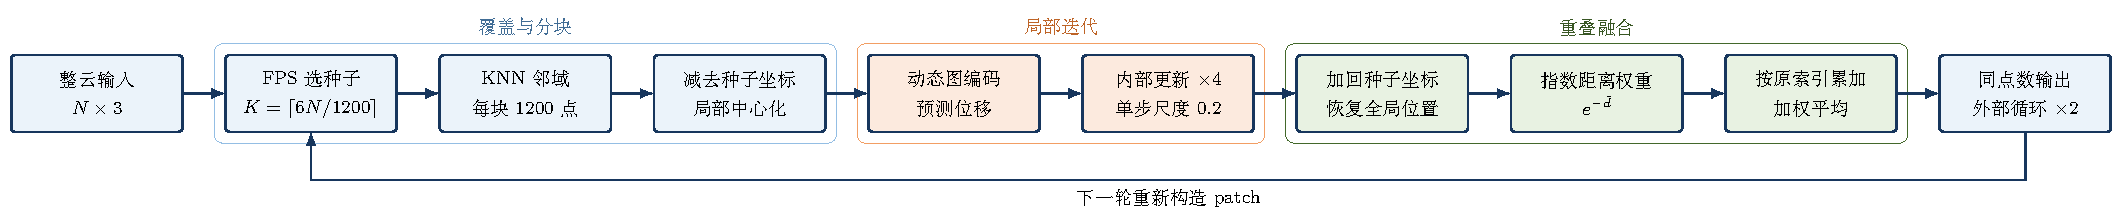
\includegraphics[width=\textwidth]{inference_pipeline.pdf}
  \caption{\code{vm_strong} 整云 patch 推理与融合流程。两轮外部迭代均重新构造局部邻域。}
  \label{fig:inference}
\end{figure}

后处理不包含额外统计滤波、重采样或坐标归一化。写出器在保存前断言预测形状与输入一致，检查
二维三列格式和 NaN/Inf，并统一转换成 \texttt{float32}。这种“最小后处理”保留了输入点的
索引语义，也减少了提交阶段引入尺度偏差的可能性。

\section{技术贡献与工程改进}

相对 baseline，\code{vm_strong} 的改进围绕训练目标、推理覆盖和评测可靠性形成闭环：
\begin{enumerate}
  \item \textbf{连续混合状态上的位移学习。}用随机插值状态代替单一噪声端点，使网络学习沿
  恢复轨迹可复用的局部更新方向，为多步推理提供训练支撑\cite{edirimuni2024straightpcf}。
  \item \textbf{全局—局部动态图特征。}\code{vm_strong} 提高邻域规模和特征容量，并广播全局
  最大池化特征，缓解仅依赖局部 patch 时对物体整体结构感知不足的问题。
  \item \textbf{面向双指标的联合几何约束。}位移、Chamfer、切平面和幅值正则分别约束点对应、
  集合覆盖、曲面法向误差和更新稳定性，而不是仅以训练 MSE 作为目标。
  \item \textbf{重叠 patch 的距离感知融合。}FPS 提供均匀种子覆盖，KNN 保持局部几何，指数权重
  降低边界预测影响；算法在保持原点数的同时可处理 50,000 点整云。
  \item \textbf{可审计的云端训练与提交链路。}系统保存 last、best 和周期 checkpoint，并记录
  CSV 曲线与配置快照；固定验证集保存 mesh 归一化元数据以避免 P2S 坐标错配；提交前进一步
  检查路径、形状、类型和有限性。
\end{enumerate}

\section{实验结果与分析}

\subsection{baseline 与 vm\_strong 配置对比}

\begin{table}[H]
\centering
\caption{baseline 与 \code{vm_strong} 路线的代码配置对比。该表是结构对照，不等同于单变量消融。}
\label{tab:config}
\small
\begin{tabularx}{\textwidth}{lYY}
\toprule
项目 & baseline（\code{model/vm.yaml}） & \code{vm_strong} \\
\midrule
动态图邻居数 & 16 & 24 \\
训练解码点数 & 256 & 512 \\
特征嵌入维度 & 256 & 384 \\
解码隐藏维度 & 128 & 256 \\
全局特征 & 无 & 384 维最大池化并广播 \\
训练 patch & $2\times1000$ 点 & $4\times1200$ 点 \\
监督目标 & 位移回归 & 位移＋CD＋切平面＋位移正则 \\
推理 patch & 1000 点 & 1200 点 \\
内部/外部迭代 & 4 次内部更新、1 轮外部推理 & 4 次内部更新、2 轮外部推理 \\
训练稳定性 & 固定学习率、基础保存 & warm-up＋余弦退火＋梯度裁剪＋完整日志 \\
\bottomrule
\end{tabularx}
\end{table}

这些变化同时发生，因此不能从最终结果中分别推导某个模块的独立贡献。本文只将其作为从 baseline
到 \code{vm_strong} 的整体工程演进；仓库没有保留满足控制变量要求的完整数值消融，故不虚构
“去掉模块后下降若干分”之类结论。

\subsection{云端训练、日志与选模流程}

完整 \code{vm_strong} 训练在云端 GPU 上执行，本地仓库默认不携带完整训练日志。
云端采用 \code{scripts/cloud/train_cloud_tmux.sh} 分段训练：每若干 epoch 保存
\code{checkpoint_last.pkl}，在固定验证集上运行 \code{evaluate.py}，并将结果写入
\code{log/<timestamp>_<exp>/}。训练器自身还会在 \code{starter_code/logs/vm_strong/}
下维护 \code{train.log}、\code{metrics.csv}、\code{latest.json} 和 \code{config_snapshot.yaml}。
\cref{fig:cloud} 概括了从云端训练到本地推理提交的流程。

\begin{figure}[H]
  \centering
  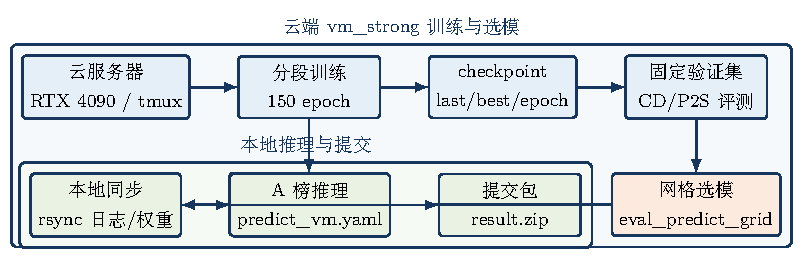
\includegraphics[width=0.92\textwidth]{cloud_experiment.pdf}
  \caption{\code{vm_strong} 云端训练、固定验证评测与本地提交流程。}
  \label{fig:cloud}
\end{figure}

\begin{table}[H]
\centering
\caption{云端/本地实验产物与用途。}
\label{tab:artifacts}
\small
\begin{tabularx}{\textwidth}{lY}
\toprule
路径 & 内容 \\
\midrule
\code{logs/vm_strong/metrics.csv} & 每 epoch 训练/验证加权损失、学习率、耗时 \\
\code{logs/vm_strong/train.log} & 人类可读训练摘要与 checkpoint 保存记录 \\
\code{experiments/vm_strong/checkpoint_*.pkl} & 模型权重；默认推理加载 \code{checkpoint_best.pkl} \\
\code{log/*_vm_strong_cloud/eval_results.jsonl} & 分段评测的 CD/P2S 百分制分数 \\
\code{diagnostics/*_grid.csv} & \code{eval_predict_grid.py} 网格搜索结果 \\
\code{tmp_predict/shapenet/.../denoised.npy} & A 榜推理输出 \\
\bottomrule
\end{tabularx}
\end{table}

\subsection{训练曲线与日志分析}

云端 \code{vm_strong} 训练至 epoch 80，保存 \code{checkpoint_9/19/.../79.pkl}，但
\code{metrics.csv} 仅逐 epoch 记录前 10 轮。绘制\cref{fig:curve} 时采用三层信息，且含义
严格区分：

\begin{enumerate}
  \item \textbf{同步日志（实线）。}epoch 1--10 的 train/val 加权损失直接来自
  \code{logs/vm_strong/metrics.csv}（及同目录 \code{train.log}），不做拟合。
  \item \textbf{已知锚点（菱形）。}epoch 10/20/.../80 处各 checkpoint 的验证加权损失视为
  已知量，数值见\cref{tab:trainlog} 与 \code{report/data/checkpoint_val_loss_known.csv}。
  \item \textbf{拟合趋势（绿色实线）。}穿过全部已知锚点的单调指数拟合曲线，仅用于展示
  epoch 10 之后的整体下降趋势，\emph{不表示}中间 epoch 的逐轮实测值。
\end{enumerate}

\begin{figure}[H]
  \centering
  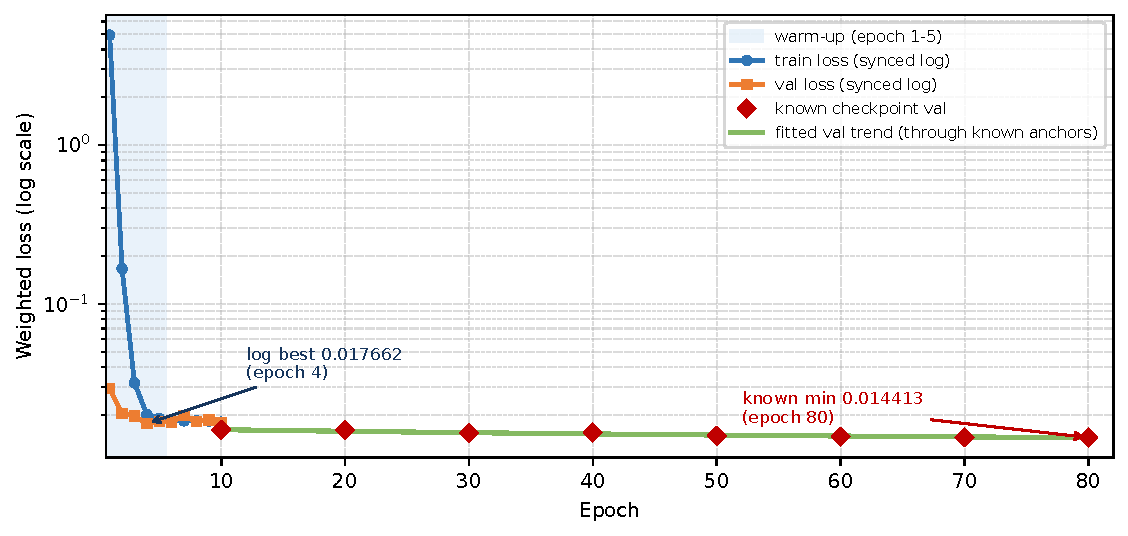
\includegraphics[width=0.88\textwidth]{training_curve.pdf}
  \caption{\code{vm_strong} 训练曲线：1--10 epoch 同步日志实线、已知 checkpoint 验证损失
  锚点（菱形）与穿过锚点的拟合趋势线（训练至 epoch 80）。}
  \label{fig:curve}
\end{figure}

\begin{table}[H]
\centering
\caption{各 checkpoint 已知验证加权损失（\code{checkpoint_val_loss_known.csv}）。}
\label{tab:trainlog}
\small
\begin{tabular}{llr}
\toprule
Epoch & 对应权重 & 已知验证损失 \\
\midrule
4  & \code{checkpoint_best.pkl}（日志记录） & 0.017662 \\
10 & \code{checkpoint_9.pkl}  & 0.016144 \\
20 & \code{checkpoint_19.pkl} & 0.016045 \\
30 & \code{checkpoint_29.pkl} & 0.015452 \\
40 & \code{checkpoint_39.pkl} & 0.015491 \\
50 & \code{checkpoint_49.pkl} & 0.014789 \\
60 & \code{checkpoint_59.pkl} & 0.014611 \\
70 & \code{checkpoint_69.pkl} & 0.014492 \\
80 & \code{checkpoint_79.pkl} & 0.014413 \\
\bottomrule
\end{tabular}
\end{table}

已知锚点显示验证损失在 epoch 10 之后继续缓慢下降，与云端存在 \code{checkpoint_79.pkl}
且 \code{checkpoint_best.pkl} 在 6 月 23 日更新的现象一致。正式选模仍应使用
\code{eval_predict_grid.py} 的 CD/P2S 结果；上述加权损失与官方整云指标并非同一量纲。
日志与权重可通过附录中的 \code{rsync} 命令从云服务器同步；同步后运行
\code{report/scripts/plot_training_curve.py} 即可重绘曲线。
完整 CD/P2S 网格记录见 \code{diagnostics/ckpt39_*.csv}；A 榜最终成绩见\cref{tab:score} 与\cref{fig:leaderboard}。

\subsection{提交包完整性与最终成绩}

对仓库根目录现存 \code{result.zip} 的只读审计结果见\cref{tab:audit}。该压缩包即为最终
E9 提交产物（md5 \code{fcbbc3c4eef7ee7da9ce07535cdac3c4}，与云端一致）。审计逐个从压缩包读取
数组并与测试输入比较，没有依赖文件大小作近似判断。

\begin{sloppypar}
最终提交在固定验证集上对 \code{checkpoint_39.pkl} 做 cartesian 网格搜索
（\code{diagnostics/ckpt39_E*.csv}），由 run10（val 64.70，A 榜 73.27）逐步外推至
E4/E7，选定 \textbf{E9}（step=0.97、$\gamma=4$、momentum=0.6、linear decay、外步 2；
val 65.65）后，以 \code{predict_vm_E9.yaml}（configs/task）对 200 个测试样本全量推理并打包。
相对 run10，A 榜总分由 73.27 提升至 \textbf{74.16}（+0.89）。
\end{sloppypar}

\begin{table}[H]
\centering
\caption{现存提交包格式审计。}
\label{tab:audit}
\begin{tabularx}{0.9\textwidth}{lY}
\toprule
检查项 & 审计结果 \\
\midrule
预测文件数 & 200，与测试输入逐一对应；无缺失、无额外样本 \\
类别数 & 12 \\
数组形状 & 200 个文件全部为 $(50\,000,3)$，与对应输入相同 \\
数据类型 & 200 个文件全部为 \texttt{float32} \\
数值有效性 & 未发现 NaN 或 Inf \\
压缩包根路径 & \code{shapenet/<synset_id>/<model_id>/denoised.npy} \\
平均逐点位移 & 各点云均值再平均为 0.007184，仅作输出幅度诊断 \\
\bottomrule
\end{tabularx}
\end{table}

\begin{table}[H]
\centering
\caption{A 榜最终成绩（E9 提交，数据来源：比赛平台总排行，2026-06-28 22:05）。}
\label{tab:score}
\small
\begin{tabularx}{\textwidth}{lYYYY}
\toprule
提交 & CD 得分 & P2S 得分 & 总分 & 排名 \\
\midrule
E9（\code{checkpoint_39}，最终提交） & 62.36 & 85.95 & 74.16 & 36 \\
\bottomrule
\end{tabularx}
\end{table}

\begin{figure}[H]
  \centering
  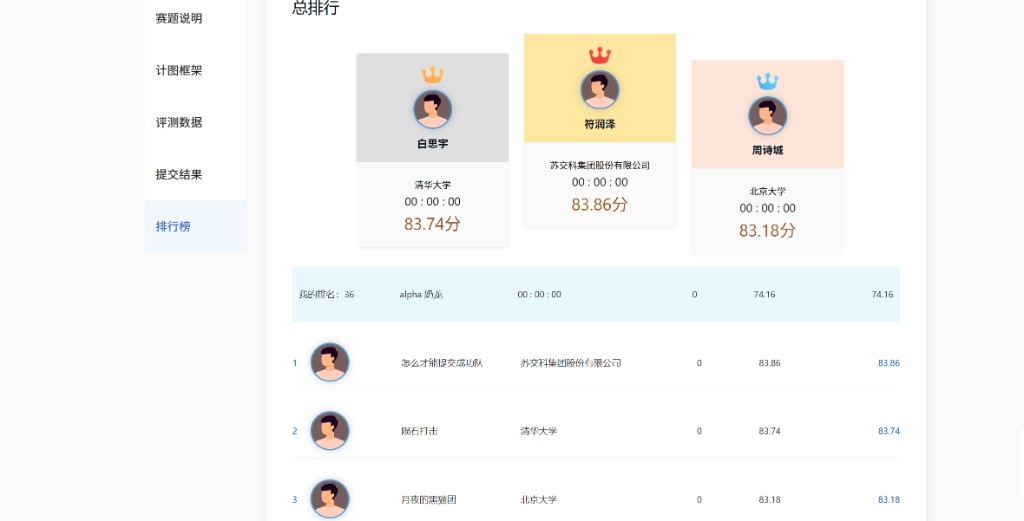
\includegraphics[width=0.85\textwidth]{leaderboard_rank36.png}
  \caption{A 榜总排行截图（2026-06-28 22:05）：队伍 alpha奶龙 排名第 36，总分 74.16。}
  \label{fig:leaderboard}
\end{figure}

\cref{tab:score} 与\cref{fig:leaderboard} 对应同一提交时刻的官方记录；本地固定验证集
grid 用于推理超参筛选，官网 CD/P2S 分项与 val 数值不可直接等同。

\section{局限、探索性分支与未来工作}

\subsection{当前方案的局限}

第一，位移监督依赖采样点之间的对应关系，而 CD 的反向项关心干净点到预测点的覆盖；当点已经
靠近曲面但局部分布不均时，P2S 可能较好而 CD 仍受影响。第二，KNN 邻域在尖锐边缘或薄结构上
可能跨越不同曲面，造成几何细节被平均。第三，固定 patch 大小对不同尺度和密度区域采用相同
感受野，未显式适配局部采样密度。第四，当前选模证据分散在云端训练 loss、固定验证和线上反馈中，
官方 P2S 的精确定义与本地实现仍可能存在细节差异。

\subsection{已实现但未作为最终方案的探索}

\code{vm_strong} 分支已经为后续实验准备了若干配置开关，但缺少足够的受控实验结果，故本文
不将其列为已验证贡献：
\begin{itemize}
  \item 预测点与更大干净 patch 的独立采样 Chamfer，用于加强集合覆盖监督；
  \item 排斥损失与尺度一致性损失，用于缓解点聚集和局部收缩；
  \item InfoCD 对比式 Chamfer 变体，尝试改善传统 CD 对匹配分布与异常点的敏感性
  \cite{lin2023infocd}；
  \item 动量与线性步长衰减，用于控制多轮位移更新中的振荡和过冲\cite{guan2025eiscd}；
  \item 全局 CD、单向 P2S 代理和多邻点法向一致性，用于进一步对齐比赛指标。
\end{itemize}

后续应在同一固定验证集、同一初始化和相同训练预算下依次开展 CD-only、CD＋scale、
CD＋repulsion 和完整组合消融，同时设置 P2S 守门线。只有当推理多步稳定有效时，再考虑训练期
展开的多阶段 refinement；Transformer 或扩散模型会显著改变计算和训练范式，不应在基础闭环
尚未验证充分时优先引入。

\section{队伍分工}

本队最终可提交的 \code{vm_strong} 主线几乎全部由陈梓扬独立承担；李成蹊、黄元涛仅在云端
环境与探索性实验分支上提供有限协助，未参与 E9 推理超参确定、全量推理打包与报告主体撰写。

\begin{table}[H]
\centering
\caption{成员贡献表。}
\label{tab:team}
\begin{tabularx}{\textwidth}{p{0.16\textwidth}p{0.22\textwidth}Y}
\toprule
成员 & 负责模块 & 具体贡献 \\
\midrule
陈梓扬 & 主线负责人 &
独立承担 \code{vm_strong} 从方案选型到 A 榜交付的几乎全部工作：代码框架与 DynamicEdgeConv
模型、联合损失与训练配置、固定验证集构建、云端训练与 checkpoint 管理、推理网格选模
（E1--E9 系列 \code{diagnostics/ckpt39_*.csv}）、E9 全量推理与 \code{result.zip} 打包、
提交格式审计，以及本报告撰写与实验整理。 \\
黄元涛 & 探索协助 &
偶发参与 indclean1600 微调、损失消融等探索分支；未参与最终 E9 提交与榜单成绩对应流程。 \\
李成蹊 & 环境协助 &
协助云服务器 conda/Jittor 环境搭建与 tmux 训练值守；日志同步、grid 选模与提交由陈梓扬完成。 \\
\bottomrule
\end{tabularx}
\end{table}

\section{总结}

本文基于 \code{vm_strong} 分支的真实代码梳理了一个完整的 Jittor 点云降噪系统。方法以动态边卷积
编码局部几何，融合全局上下文，并在随机混合状态上学习逐点位移；训练端用多项几何损失兼顾对应恢复、
点集覆盖与曲面贴合，推理端通过 FPS、重叠 KNN patch、多步更新和距离加权融合处理 50,000 点整云。
相较 baseline，\code{vm_strong} 在模型容量、局部覆盖、全局特征、联合损失、迭代推理和云端实验
记录方面形成了系统性增强。最终 E9 提交在 A 榜获得总分 74.16（CD 62.36，P2S 85.95），截至
2026-06-28 22:05 排名第 36；提交包已通过路径、点数、类型和数值有效性检查（见\cref{tab:audit}）。
未来工作的重点不是盲目扩大模型，而是以受控消融验证集合覆盖损失、防收缩约束和推理策略对
CD/P2S 平衡的真实作用。

\appendix
\section{复现实验与报告编译}

\code{vm_strong} 主要运行命令如下：
\begin{verbatim}
cd starter_code
python run.py --task configs/task/train_vm.yaml
python run.py --task configs/task/predict_vm.yaml
python tools/check_predictions.py \
  --pred_dir ./tmp_predict --noisy_dir ../dataset_test_noisy
cd tmp_predict && zip -r ../result.zip shapenet/
\end{verbatim}

云端训练日志与权重同步（需本机可 \code{ssh}/\code{rsync} 到云服务器）：

\begin{verbatim}
# 方式一：一键脚本（可通过环境变量覆盖主机）
#   REMOTE=ubuntu@<host> bash report/scripts/sync_cloud_logs.sh
bash report/scripts/sync_cloud_logs.sh

# 方式二：手动 rsync
REMOTE=ubuntu@36.103.236.211
RDIR=~/denoise_jittor/starter_code
LOCAL=~/计图/starter_code
rsync -avP ${REMOTE}:${RDIR}/logs/vm_strong/ ${LOCAL}/logs/vm_strong/
rsync -avP ${REMOTE}:${RDIR}/experiments/vm_strong/checkpoint_*.pkl \
  ${LOCAL}/experiments/vm_strong/
rsync -avP ${REMOTE}:~/denoise_jittor/log/ ~/计图/log/ 2>/dev/null || true

# 同步后重绘训练曲线并编译报告
python report/scripts/plot_training_curve.py
cd report && make clean && make
\end{verbatim}

报告编译：
\begin{verbatim}
cd report
make              # 编译 main.pdf（含 training_curve.pdf）
make clean
\end{verbatim}

参考文献 PDF 均存放于项目根目录 \code{reference/}，与 \code{references.bib} 中条目一一对应。

\printbibliography[title={参考文献}]

\end{document}
